\documentclass[11pt]{article}
\usepackage{graphicx}
\usepackage{geometry}
\usepackage{float}
\usepackage{amsmath}
\usepackage{circuitikz}
\usepackage{amssymb}
\usepackage{mathtools}
\usepackage{tikz}
\usepackage{tikz-3dplot}
\usepackage{cite}
\DeclarePairedDelimiter{\set}{\{}{\}}

\title{Magnetic Torque Investigations}
\author{Spandan Suthar and Timo Peschken}
\date{October 21, 2025}

\geometry{margin=1in}
\setlength{\parindent}{0pt}

\begin{document}

\maketitle

\section{Introduction and Background}

Magnetic dipoles are involved in a variety of phenomena in quantum
mechanics and particle physics. Their precession in a magnetic field
provides the fundamental mechanism for nuclear magnetic resonance
(NMR), used in applications from molecular structure analysis to
magnetic resonance imaging (MRI) \cite{harris, young}. Magnetic
dipole precession
contextualizes prototypical problems representative of central
quantum phenomena, such as the Zeeman effect \cite{harris}. This
experiment seeks
to investigate typical magnetic dipole behaviors associated with
torques produced by external magnetic fields. Based on a
dipole's simple harmonic motion and precession in a magnetic field,
experimental values of the dipole strength are obtained. A qualitative
investigation of the spin flip mechanism central to NMR is also
conducted.

\vspace{1em}

Consider a dipole placed in a magnetic field with some orientation
angle $\alpha$ measured from the dipole vector to the field vector. This dipole
experiences a torque $\vec \tau$ defined by:

\begin{equation}
  \vec{\tau} = \vec{\mu} \times \vec{B} = \mu B \sin \alpha
  \label{eq:magnetic_dipole_torque}
\end{equation}

where $\vec{\mu}$ represents the magnetic dipole moment and $\vec{B}$
is the external magnetic field vector \cite{young}. When the dipole
is positioned with some
angular displacement $\gamma = -\alpha$ measured from $\vec B$ to
$\vec \mu$, the torque produced by the field opposes
the initial displacement. This restoring torque is approximately proportional
to the displacement for small $\alpha$, making the motion in the
small-$\alpha$ regime simple harmonic \cite{diffeq}. In this regime, Newton's
second law for torques gives \cite{young}:

\begin{equation}
  \tau  = \mu B \sin \alpha  = - \mu B \sin \gamma \Rightarrow
  \frac{d^2\gamma}{dt^2} = -\frac{\mu B}{I} \gamma
\end{equation}

This is the equation of motion for simple harmonic motion with an
angular frequency $\omega$ satisfying \cite{diffeq}:

\begin{equation}
  \omega ^2 = \left ( \frac{2\pi}{T} \right )^2 =  \mu \cdot \frac{B}{I}
  \label{eq:sho_lr}
\end{equation}

where in general the relationship between the angular frequency and
the period of simple harmonic oscillatory motion is given by \cite{diffeq}:

\begin{equation}
  \omega = \frac{2\pi}{T}
  \label{eq:omega_period}
\end{equation}

\vspace{1em}

Another typical behavior of magnetic dipoles in magnetic fields is
precession. Magnetic precession arises when an object has a magnetic
dipole $\vec \mu$ parallel to the object's angular momentum $\vec L$
in a non-parallel magnetic field $\vec B$ \cite{young, harris}.
In this situation,
\eqref{eq:magnetic_dipole_torque} dictates that the torque experienced by
the dipole is orthogonal to the object's angular momentum and to the
magnetic field $\vec B$. This causes the angular momentum vector to change
direction with a constant rate and locks the change in angular
momentum $\Delta \vec L = \vec \tau \Delta t = \frac{d\vec L}{d t}
\Delta t$ to the
plane orthogonal
to $\vec B$, as in Figure \ref{fig:dipole_angular_momentum_3d}.

\begin{figure}[H]
  \centering
  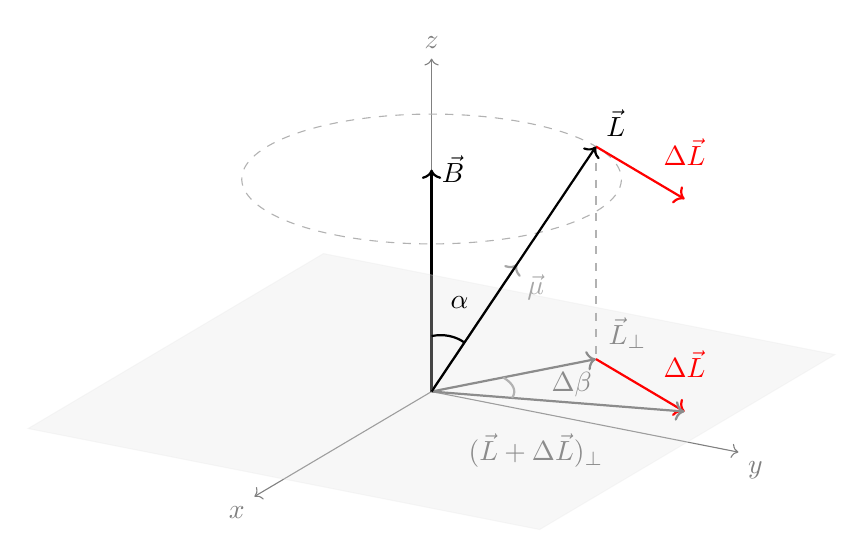
\begin{tikzpicture}[scale=1.5]
    % Set viewing angles
    \tdplotsetmaincoords{70}{120}
    \begin{scope}[tdplot_main_coords]
      % Draw coordinate axes
      \draw[gray,->] (0,0,0) -- (3,0,0) node[anchor=north east]{$x$};
      \draw[gray,->] (0,0,0) -- (0,3,0) node[anchor=north west]{$y$};
      \draw[gray,->] (0,0,0) -- (0,0,3) node[anchor=south]{$z$};
      % Vertical magnetic field vector along z-axis
      \draw[thick, black, ->] (0,0,0) -- (0,0,2.0) node[right] {$\vec{B}$};
      % Define the angle for L vector (in spherical coordinates)
      \def\theta{40}
      \def\phi{150}
      \def\Lradius{2.5}
      \def\muradius{1.3}
      % Calculate coordinates
      \pgfmathsetmacro{\Lx}{\Lradius*sin(\theta)*cos(\phi)}
      \pgfmathsetmacro{\Ly}{\Lradius*sin(\theta)*sin(\phi)}
      \pgfmathsetmacro{\Lz}{\Lradius*cos(\theta)}
      \pgfmathsetmacro{\mux}{\muradius*sin(\theta)*cos(\phi)}
      \pgfmathsetmacro{\muy}{\muradius*sin(\theta)*sin(\phi)}
      \pgfmathsetmacro{\muz}{\muradius*cos(\theta)}

      % Calculate the radius of the circle in the xy-plane
      \pgfmathsetmacro{\LxyRadius}{sqrt(\Lx*\Lx + \Ly*\Ly)}

      % Draw the orthogonal plane (perpendicular to B)
      \filldraw[gray!20, opacity=0.3] (-2.5,-2.5,0) -- (2.5,-2.5,0)
      -- (2.5,2.5,0) -- (-2.5,2.5,0) -- cycle;

      % Draw the circle parallel to xy-plane passing through the tip of L
      \draw[dashed, gray!60] (0,0,\Lz) circle (\LxyRadius);

      % Magnetic dipole moment vector parallel to angular momentum
      \draw[thick, gray!70, ->] (0,0,0) -- (\mux,\muy,\muz) node[below
      right] {$\vec{\mu}$};

      % Projection of L onto the orthogonal plane
      \draw[thick, dashed, gray!60] (\Lx,\Ly,\Lz) -- (\Lx,\Ly,0);
      \draw[thick, gray!90, ->] (0,0,0) -- (\Lx,\Ly,0)
      node[right=0.4cm,above=0.001cm]
      {$\vec{L}_{\perp}$};

      % Calculate ΔL vector as μ × B
      \def\deltaLlength{1.5}
      \pgfmathsetmacro{\normFactor}{sqrt(\muy*\muy + \mux*\mux)}
      \pgfmathsetmacro{\deltaLx}{\deltaLlength*\muy/\normFactor}
      \pgfmathsetmacro{\deltaLy}{-\deltaLlength*\mux/\normFactor}

      % Draw ΔL vector - proportional to μ × B - with label moved further away
      \draw[thick, red, ->] (\Lx,\Ly,\Lz) --
      (\Lx+\deltaLx,\Ly+\deltaLy,\Lz) node[above=0.3cm] {$\Delta \vec{L}$};

      % Draw duplicate ΔL vector in xy plane at tip of L_perp with
      % matching label position
      \draw[thick, red, ->] (\Lx,\Ly,0) --
      (\Lx+\deltaLx,\Ly+\deltaLy,0) node[above=0.3cm] {$\Delta
      \vec{L}$};

      \draw[thick, gray!90, ->] (0,0,0) --
      (\Lx+\deltaLx,\Ly+\deltaLy,0) node[below=0.5cm, left=0.9cm]
      {$(\vec{L} + \Delta \vec{L})_\perp$};

      % Angular momentum vector
      \draw[thick, black, ->] (0,0,0) -- (\Lx,\Ly,\Lz) node[above
      right] {$\vec{L}$};

      % Arc showing angle between B and L
      % Draw the arc WITHOUT a label first
      \tdplotsetthetaplanecoords{\phi}
      \tdplotdrawarc[tdplot_rotated_coords,thick,black]{(0,0,0)}{0.5}{0}{\theta}{}{}

      % Calculate a position for the alpha symbol
      \pgfmathsetmacro{\labelR}{0.8}
      \pgfmathsetmacro{\labelTheta}{\theta/2}
      \pgfmathsetmacro{\labelX}{\labelR*sin(\labelTheta)*cos(\phi)}
      \pgfmathsetmacro{\labelY}{\labelR*sin(\labelTheta)*sin(\phi)}
      \pgfmathsetmacro{\labelZ}{\labelR*cos(\labelTheta)}

      % Place the symbolic alpha instead of theta
      \node at (\labelX,\labelY,\labelZ) {$\alpha$};

      % Draw the beta arc in the xy-plane
      % Calculate angular positions of L_perp and (L+ΔL)_perp vectors
      % in the xy-plane
      \pgfmathsetmacro{\angleLperp}{atan2(\Ly,\Lx)}
      \pgfmathsetmacro{\angleLplusDL}{atan2(\Ly+\deltaLy,\Lx+\deltaLx)}

      % Draw arc showing beta angle between L_perp and (L+ΔL)_perp
      \draw[thick, gray!60] (0,0,0) + ({\angleLperp}:0.7) arc
      ({\angleLperp}:{\angleLplusDL}:0.7);

      % Place the beta symbol in the middle of the arc
      \pgfmathsetmacro{\betaAngle}{0.5*(\angleLperp+\angleLplusDL)}
      \pgfmathsetmacro{\betaLabelX}{1.2*cos(\betaAngle)}
      \pgfmathsetmacro{\betaLabelY}{1.2*sin(\betaAngle)}
      \node[gray!90] at (\betaLabelX,\betaLabelY,0) {$\Delta \beta$};
    \end{scope}
  \end{tikzpicture}
  \caption{The angular momentum $\vec L$ and magnetic dipole moment $\vec \mu$
    of an object experiencing precession in a magnetic field $\vec
    B$. Note the circular path of the
    tip of $\vec L$, to which the change in angular momentum $\Delta
    \vec L$ caused by
    the magnetic field torque is tangent. Also note the projection of
    $\vec L$ onto the
    plane orthogonal to $\vec B$, $\vec L_\perp$; the projection of
    $(\vec L + \Delta \vec L)$ onto the same plane, $(\vec L + \Delta
    \vec L)_\perp$; and the angle $\Delta \beta$ between them. The dipole moment
  is oriented with an angle $\alpha$ with the magnetic field.}
  \label{fig:dipole_angular_momentum_3d}
\end{figure}

\vspace{1em}

% Define the change in precession angle
% Define the precession angular velocity

Consider the projection of the object's angular momentum $\vec
L_\perp$ into the plane orthogonal to the magnetic field, with magnitude
given by $L \sin \alpha$. Also consider the projection
of the angular momentum after a small change in time $\Delta t$:
$(\vec L + \Delta \vec L)_\perp$. The angle between these is $\Delta
\beta$, a change in the angle of precession $\beta$ of the object. Considering
$\Delta \beta$ to be small and noting the right triangle formed by
$\vec L_\perp$, $(\vec L + \Delta \vec L)_\perp$, and $\Delta \vec L$, a
relationship between the precession
angular frequency $\omega_p = \frac{d\beta}{dt}$, the spin angular
frequency $\omega_s$, and the angle from the magnetic field $\alpha$
is obtained:

\begin{align}
  \Delta L = L \sin \alpha \sin \Delta \beta
  \Rightarrow \frac{dL}{dt} = L \frac{d\beta}{dt} \sin \alpha
  \Rightarrow \tau = I \omega_s \omega_p \sin \alpha
\end{align}

With equations \eqref{eq:magnetic_dipole_torque} and
\eqref{eq:omega_period}, this provides a relationship between the
period $T_s$ of the object's motion about its angular
momentum axis, the angular frequency $\omega_s$ of the object's motion
about its angular momentum axis, the period $T_p$ of
precession, the angular frequency $\omega_p$ of precession, the
object's moment of inertia $I$, the dipole strength
$\mu$, and the magnetic field strength $B$:
\begin{equation}
  \omega_s \omega_p =
  \frac{(2 \pi)^2}{T_pT_s} = \mu \cdot \frac{B}{I}
  \label{eq:prec_lr}
\end{equation}

Note the symmetry with \eqref{eq:sho_lr}.

\section{Methodology}

A magnetic dipole with known dipole direction but unknown dipole
strength $\mu$ is constructed. A
time-invariant magnetic field $\vec B$ that the dipole is placed
in is produced by two twin magnetic coils, as shown in Figure
\ref{fig:apparatus}. The strength of $\vec B$ is
controlled by the current through the coils \cite{young} and measured directly
with a Gaussmeter at the
dipole's position. Dissipative forces due to contact between the
dipole and a holder for the dipole are mitigated with a cushion of
compressed air,
allowing the dipole to
rotate freely. The moment of inertia $I$ of the dipole is estimated as that
of a solid sphere of mass $m = 183.0 \pm 0.1$ g and radius $r = 28.5
\pm 3$ mm \cite{young}.

\begin{figure}[H]
  \centering
  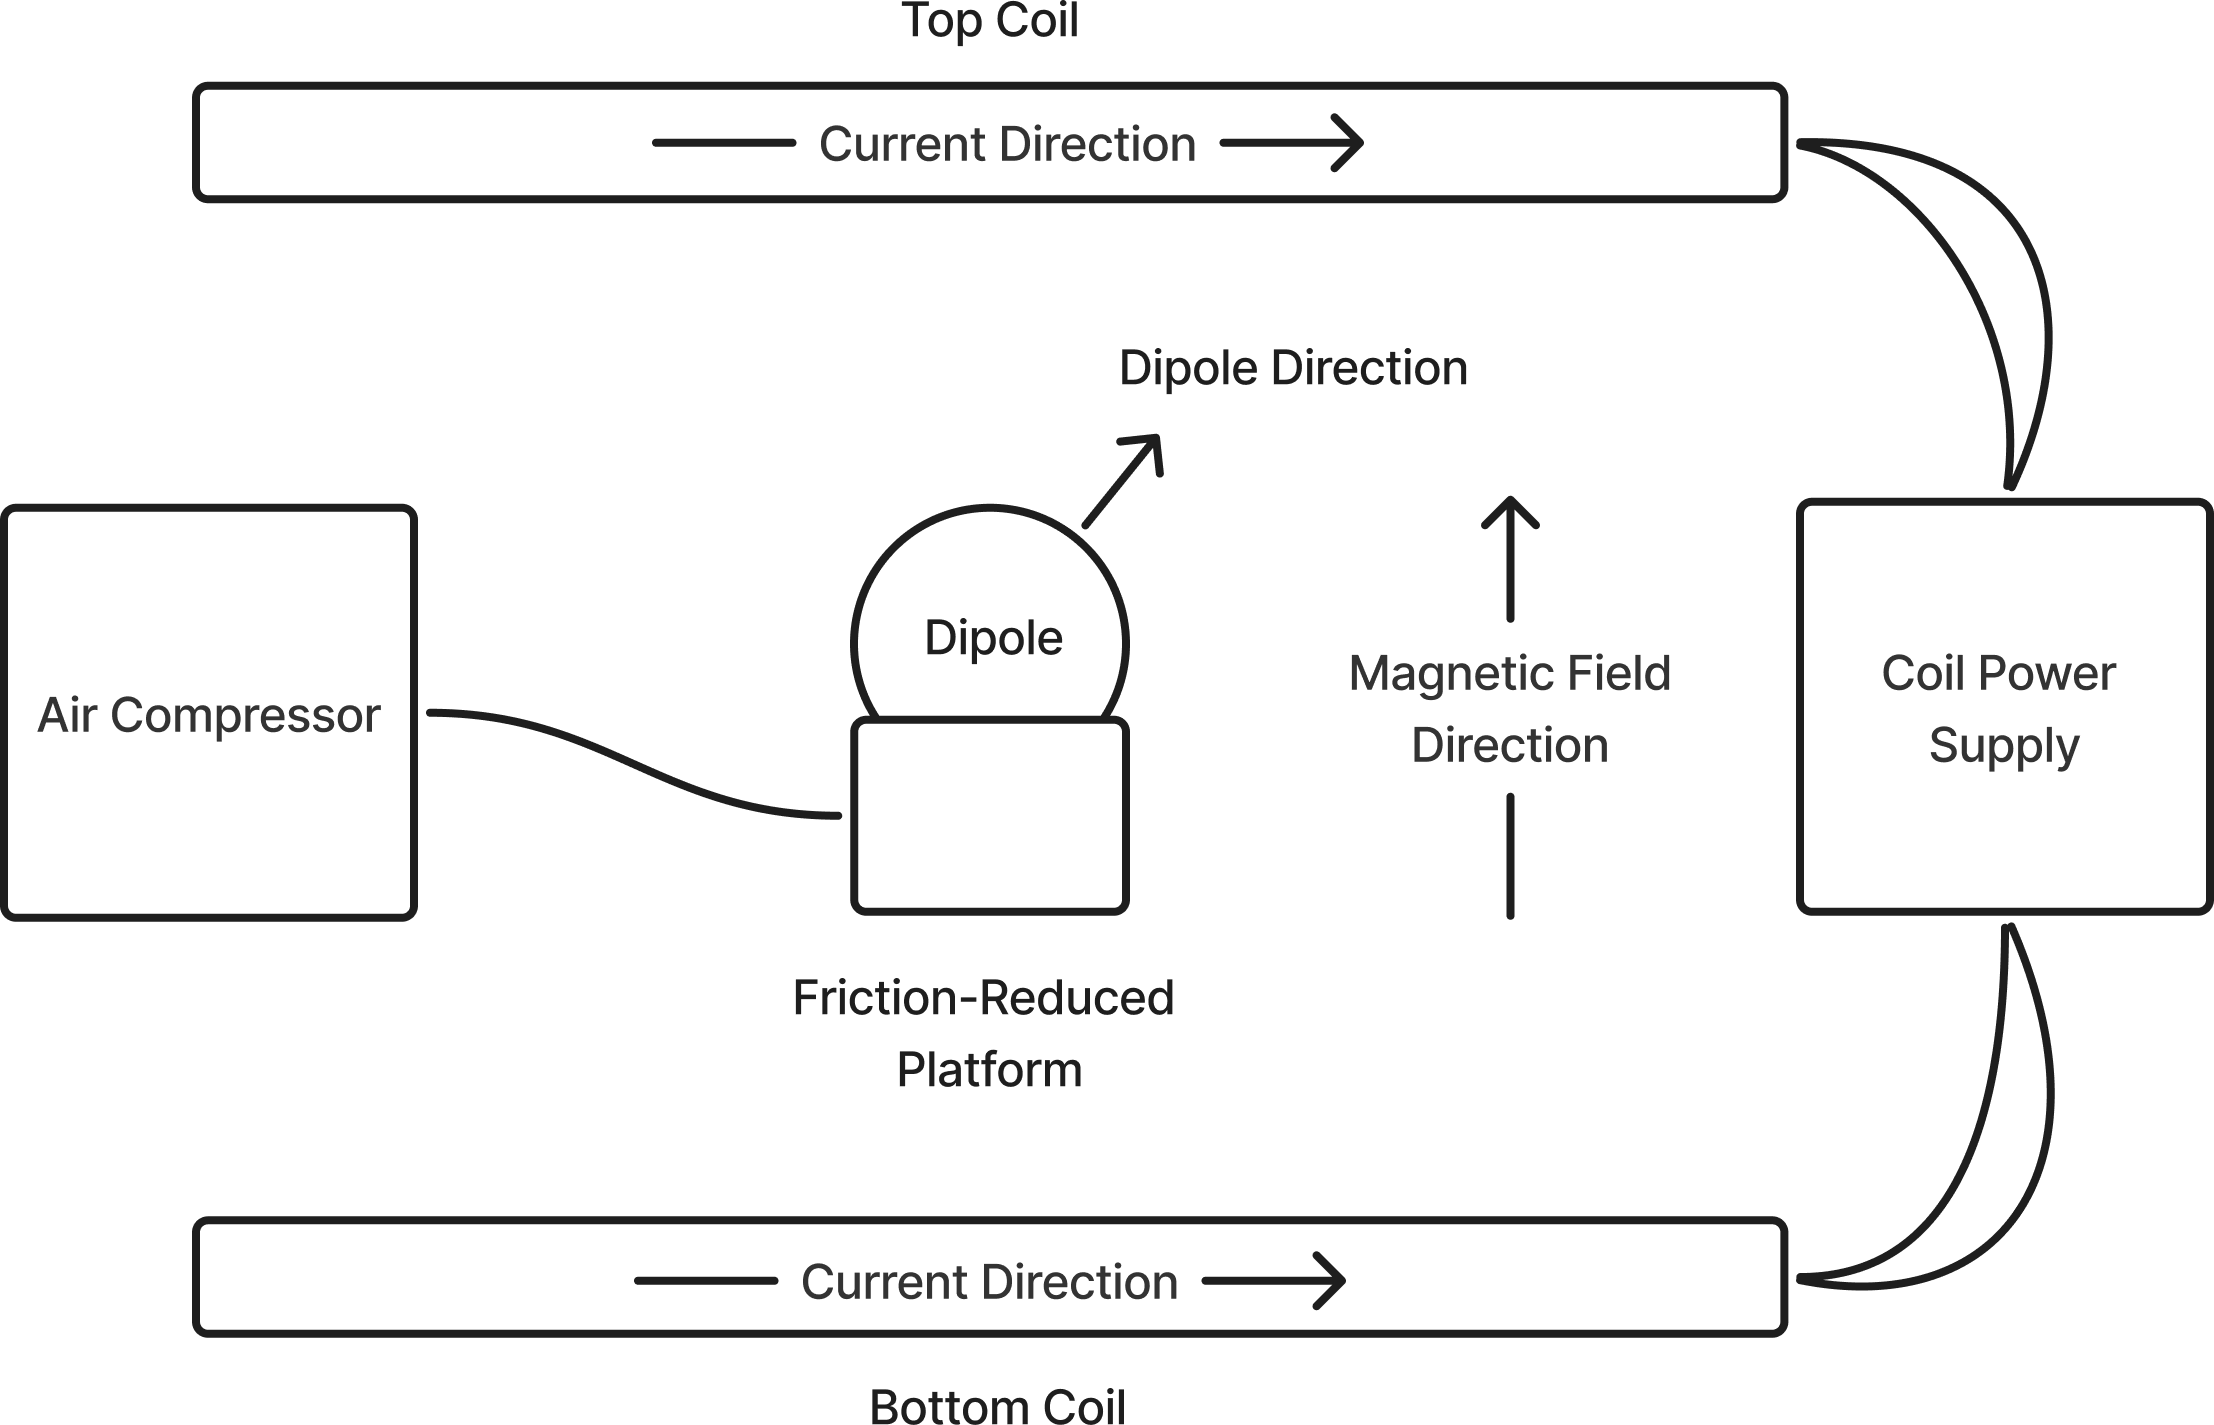
\includegraphics[width=0.7\textwidth]{../coils.png}
  \caption{Experimental apparatus for the three magnetic dipole
    experiments. The dipole platform
    sits between two magnetic coils, producing an upward magnetic
    field due their agreeing currents (supplied by a DC power supply).
  An air compressor provides a low-friction cushion for the dipole.}
  \label{fig:apparatus}
\end{figure}

The unknown strength of the dipole is measured using two experiments:
an experiment of simple harmonic motion and an experiment of
magnetic precession.

\subsection{Simple Harmonic Motion}

At each current in Table \ref{tab:results}, the dipole is placed on
its holder with $\vec \mu$ aligned with $\vec B$ and given a small
initial angular displacement $\alpha_0$ about $\vec B$. It is then
allowed to oscillate and the
average period across five oscillation cycles is measured with a clock.
This five-oscillation average is repeated five times; another average is
taken over these repetitions to obtain a final period of oscillation $T$.

\subsection{Magnetic Precession}

At each current in Table \ref{tab:results}, the dipole is placed upon its
holder with $\vec \mu$ oriented at an angle $\alpha$ away
from the vertical. The dipole is then given a modest angular velocity
$\omega_s$ (period $T_s$) about its dipole axis. Precession results,
and the precession period $T_p$
is obtained as an average over half a precession cycle. $\omega_s$ is
derived from an average between readings from a tachometer taken at the start
and end of this half-cycle. Note that only half a
cycle is considered to minimize energy loss of the dipole due to air
resistance.

\subsection{Spin Flip Mechanism}

A brief exploration of the spin flip mechanism is also conducted. As in the
precession experiment, the dipole is placed upon its holder with an
initial angular velocity and allowed to precess. Two magnets are then
placed on either
side of the dipole and rotated so as to appear motionless in the dipole's
precessing frame of
reference, producing a magnetic field that is constantly perpendicular to the
dipole as it precesses. It is observed that the dipole flips its
orientation under the torque caused by the external magnetic field,
in the direction predicted by
equation \eqref{eq:magnetic_dipole_torque}.

\section{Results}

Data points for magnetic fields corresponding to all currents are
presented in Table \ref{tab:results}. Equations \eqref{eq:sho_lr} and
\eqref{eq:prec_lr} suggest that plotting $\left ( \frac{2\pi}{T} \right )^2$
and $ \frac{(2\pi)^2}{T_p T_s}$ against $\frac{B}{I}$,
respectively,
should yield linear relationships whose slopes yield two experimental
value of the dipole
strength $\mu$. These relationships from the experimental data are plotted
in Figures \ref{fig:sho_lr_plot} and \ref{fig:prec_lr_plot} and
linear regression is performed, yielding $\mu$-values of
$(1.63 \pm 0.08)$ A $\cdot$ m$^2$ and $(1.47 \pm 0.13)$ A $\cdot$
m$^2$, respectively. These values are consistent with each other to
within 1$\sigma$.

% \begin{table}[H]
%   \centering
%   \begin{tabular}{c c c c}
%     \hline
%     Current (A) ($\pm$ 0.01 A) & SHO Period (s) & Spin Period (s) &
%     Precession Period (s) \\
%     \hline
%     2.00 & $1.020 \pm 0.009$ & $0.0590 \pm 0.0012$ & 23.1 \\
%     1.75 & $1.134 \pm 0.015$ & $0.062 \pm 0.003$ & 24.2 \\
%     1.50 & $1.221 \pm 0.016$ & $0.0646 \pm 0.0028$ & 30.4 \\
%     1.25 & $1.365 \pm 0.022$ & $0.0578 \pm 0.0024$ & 43.2 \\
%     1.00 & $1.502 \pm 0.008$ & $0.074 \pm 0.003$ & 46.9 \\
%     \hline
%   \end{tabular}
%   \caption{Measured values of the simple harmonic motion period $T$,
%   spin period $T_s$, and precession period $T_p$ for each coil
% current tested.}
%   \label{tab:results}
% \end{table}

\begin{table}[H]
  \centering
  \begin{tabular}{c c c c c}
    \hline
    Current (A) ($\pm$ 0.01 A) & $T$ (s) & $T_s$ (s) &
    $T_p$ (s) ($\pm$ 1 s) & B ($10^{-3}$ T) ($\pm 10^{-5}$ T) \\
    \hline
    2.00 & $1.020 \pm 0.009$ & $0.0590 \pm 0.0012$ & 23.1 & $1.39
    $ \\
    1.75 & $1.134 \pm 0.015$ & $0.062 \pm 0.003$ & 24.2 & $1.17 $ \\
    1.50 & $1.221 \pm 0.016$ & $0.0646 \pm 0.0028$ & 30.4 & $1.01
    $ \\
    1.25 & $1.365 \pm 0.022$ & $0.0578 \pm 0.0024$ & 43.2 & $0.83
    $ \\
    1.00 & $1.502 \pm 0.008$ & $0.074 \pm 0.003$ & 46.9 & $0.64
    $ \\
    \hline
  \end{tabular}
  \caption{Measured values of the simple harmonic motion period $T$,
    spin period $T_s$, precession period $T_p$, and magnetic field strength $B$
  for each coil current tested.}
  \label{tab:results}
\end{table}

\begin{figure}[H]
  \centering
  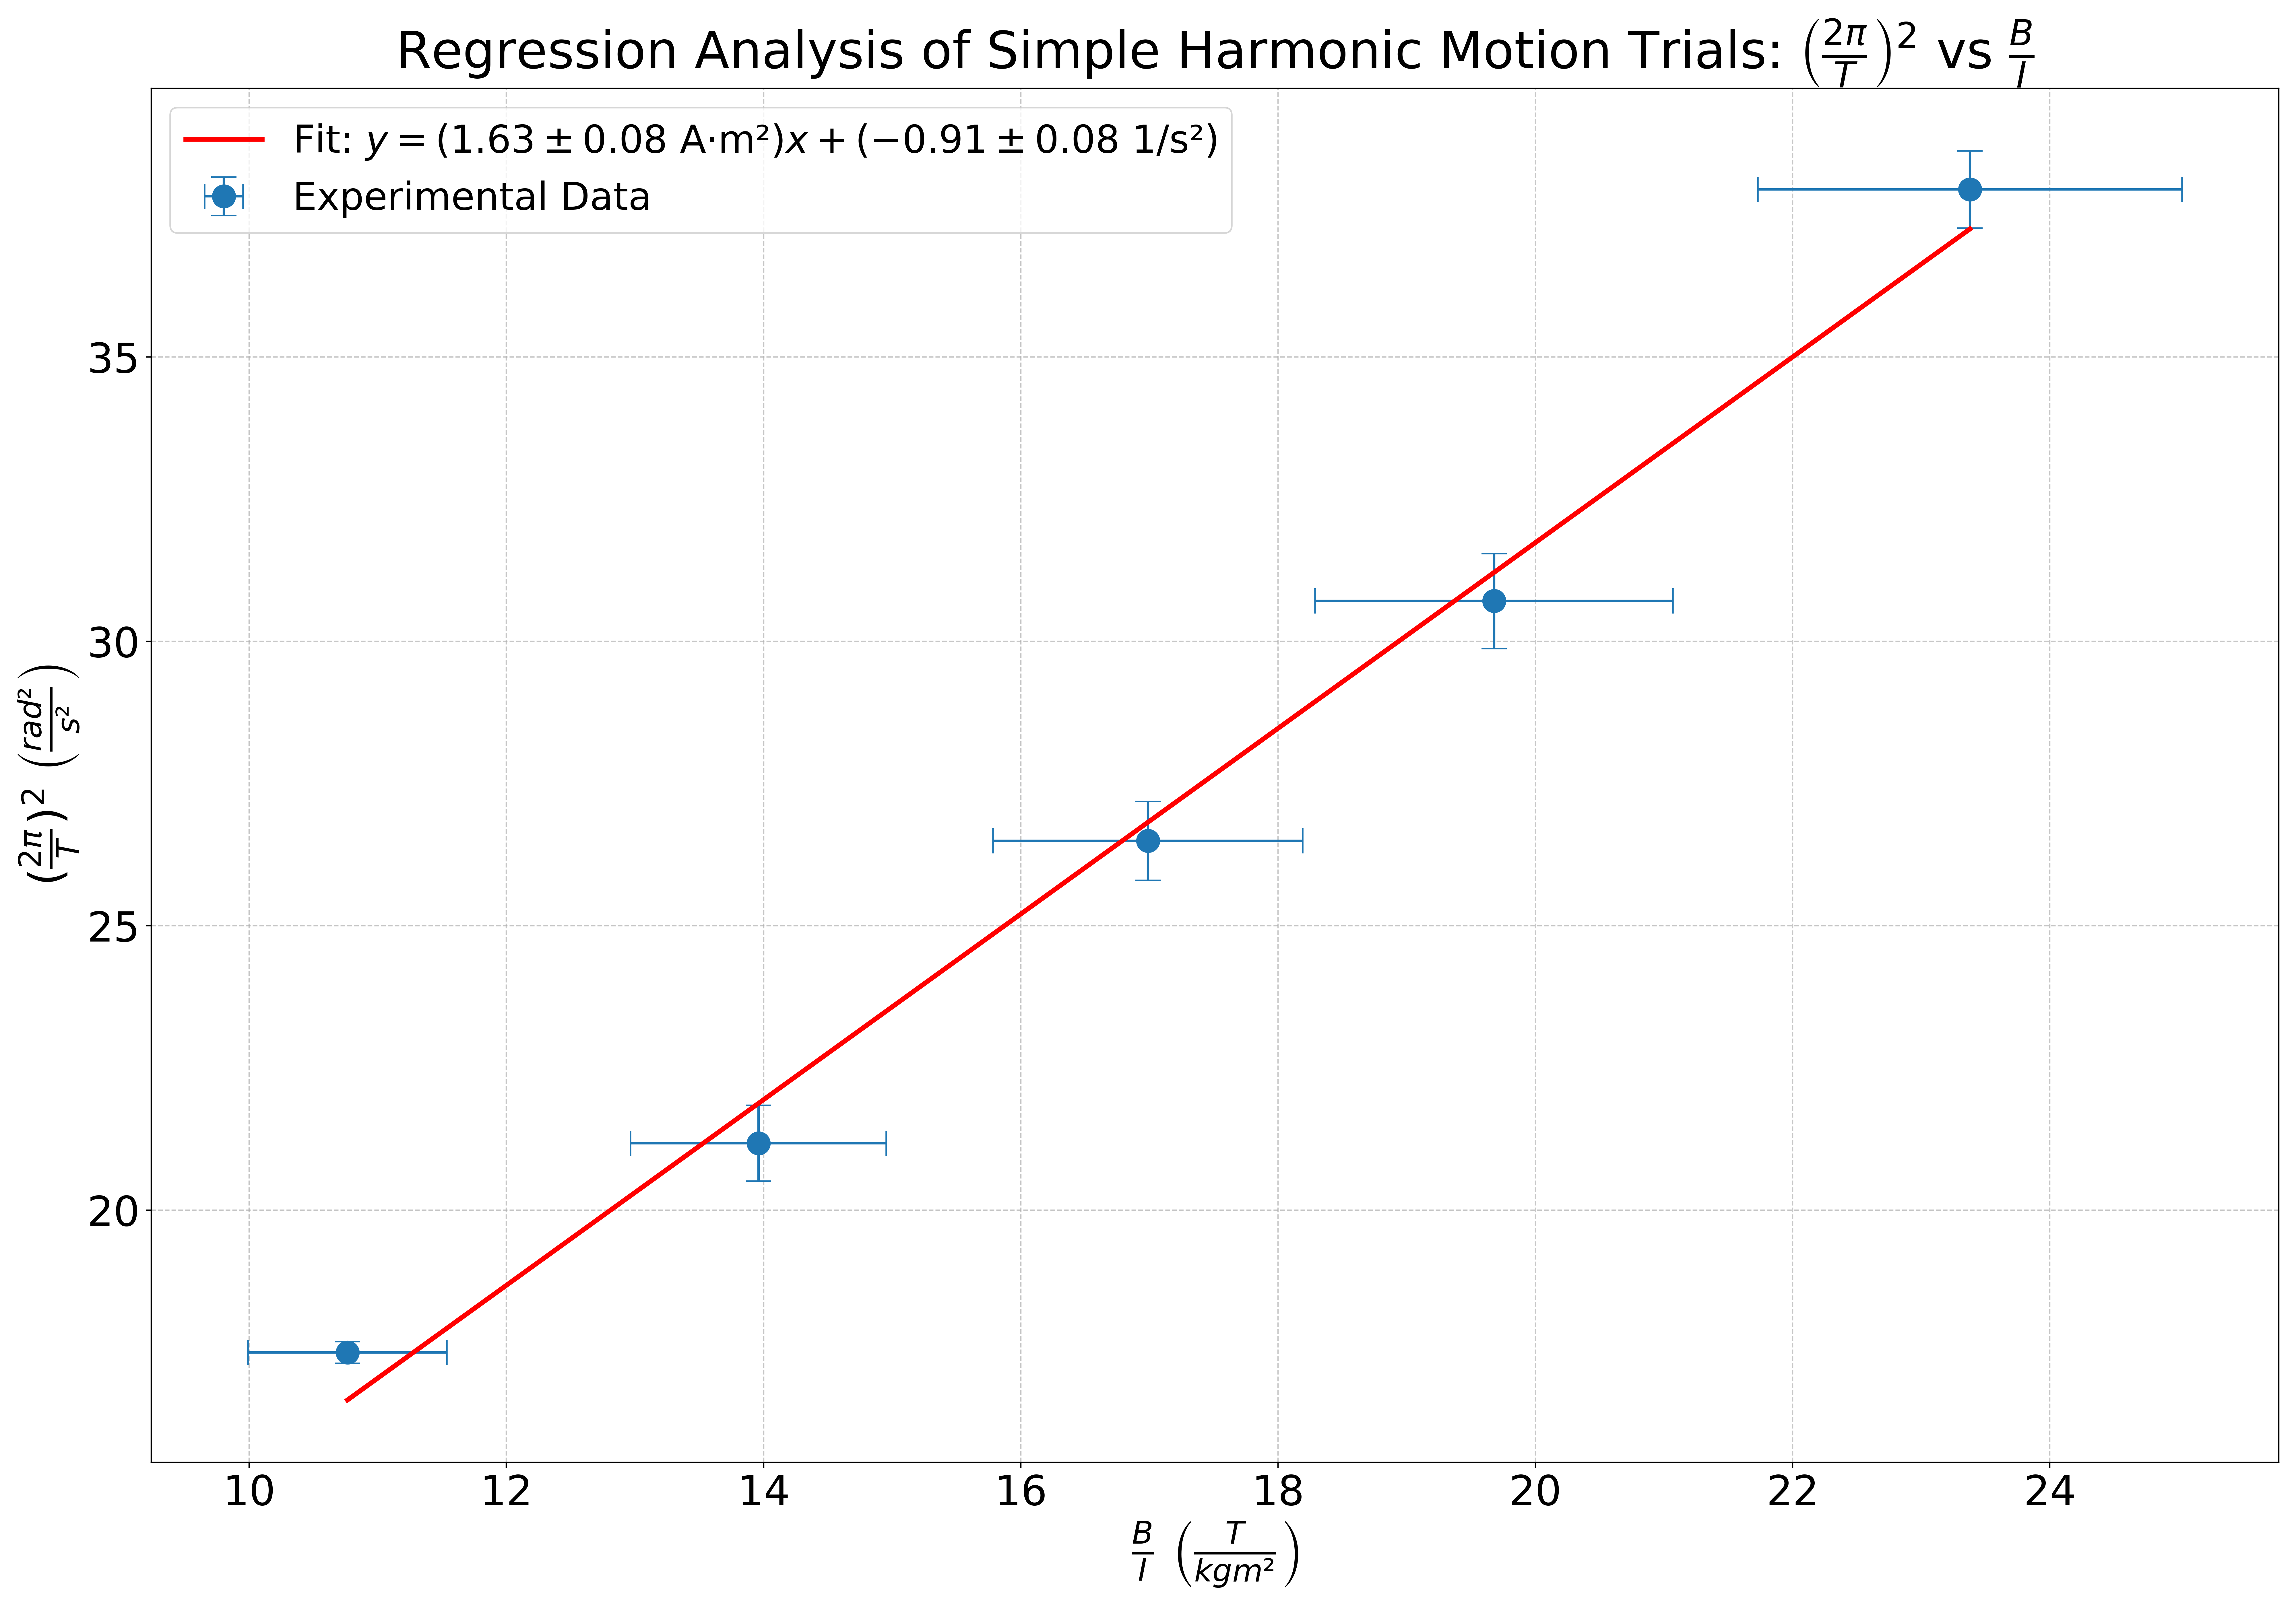
\includegraphics[width=1.0\textwidth]{../simple_harmonic_motion_trials.png}
  \caption{A plot of $\left ( \frac{2\pi}{T} \right )^2$ against
    $\frac{B}{I}$ for the simple harmonic motion experiment.
    The linear regression fit is shown in red, with associated data
  points from Table \ref{tab:results} in blue. Origin not shown.}
  \label{fig:sho_lr_plot}
\end{figure}

\begin{figure}[H]
  \centering
  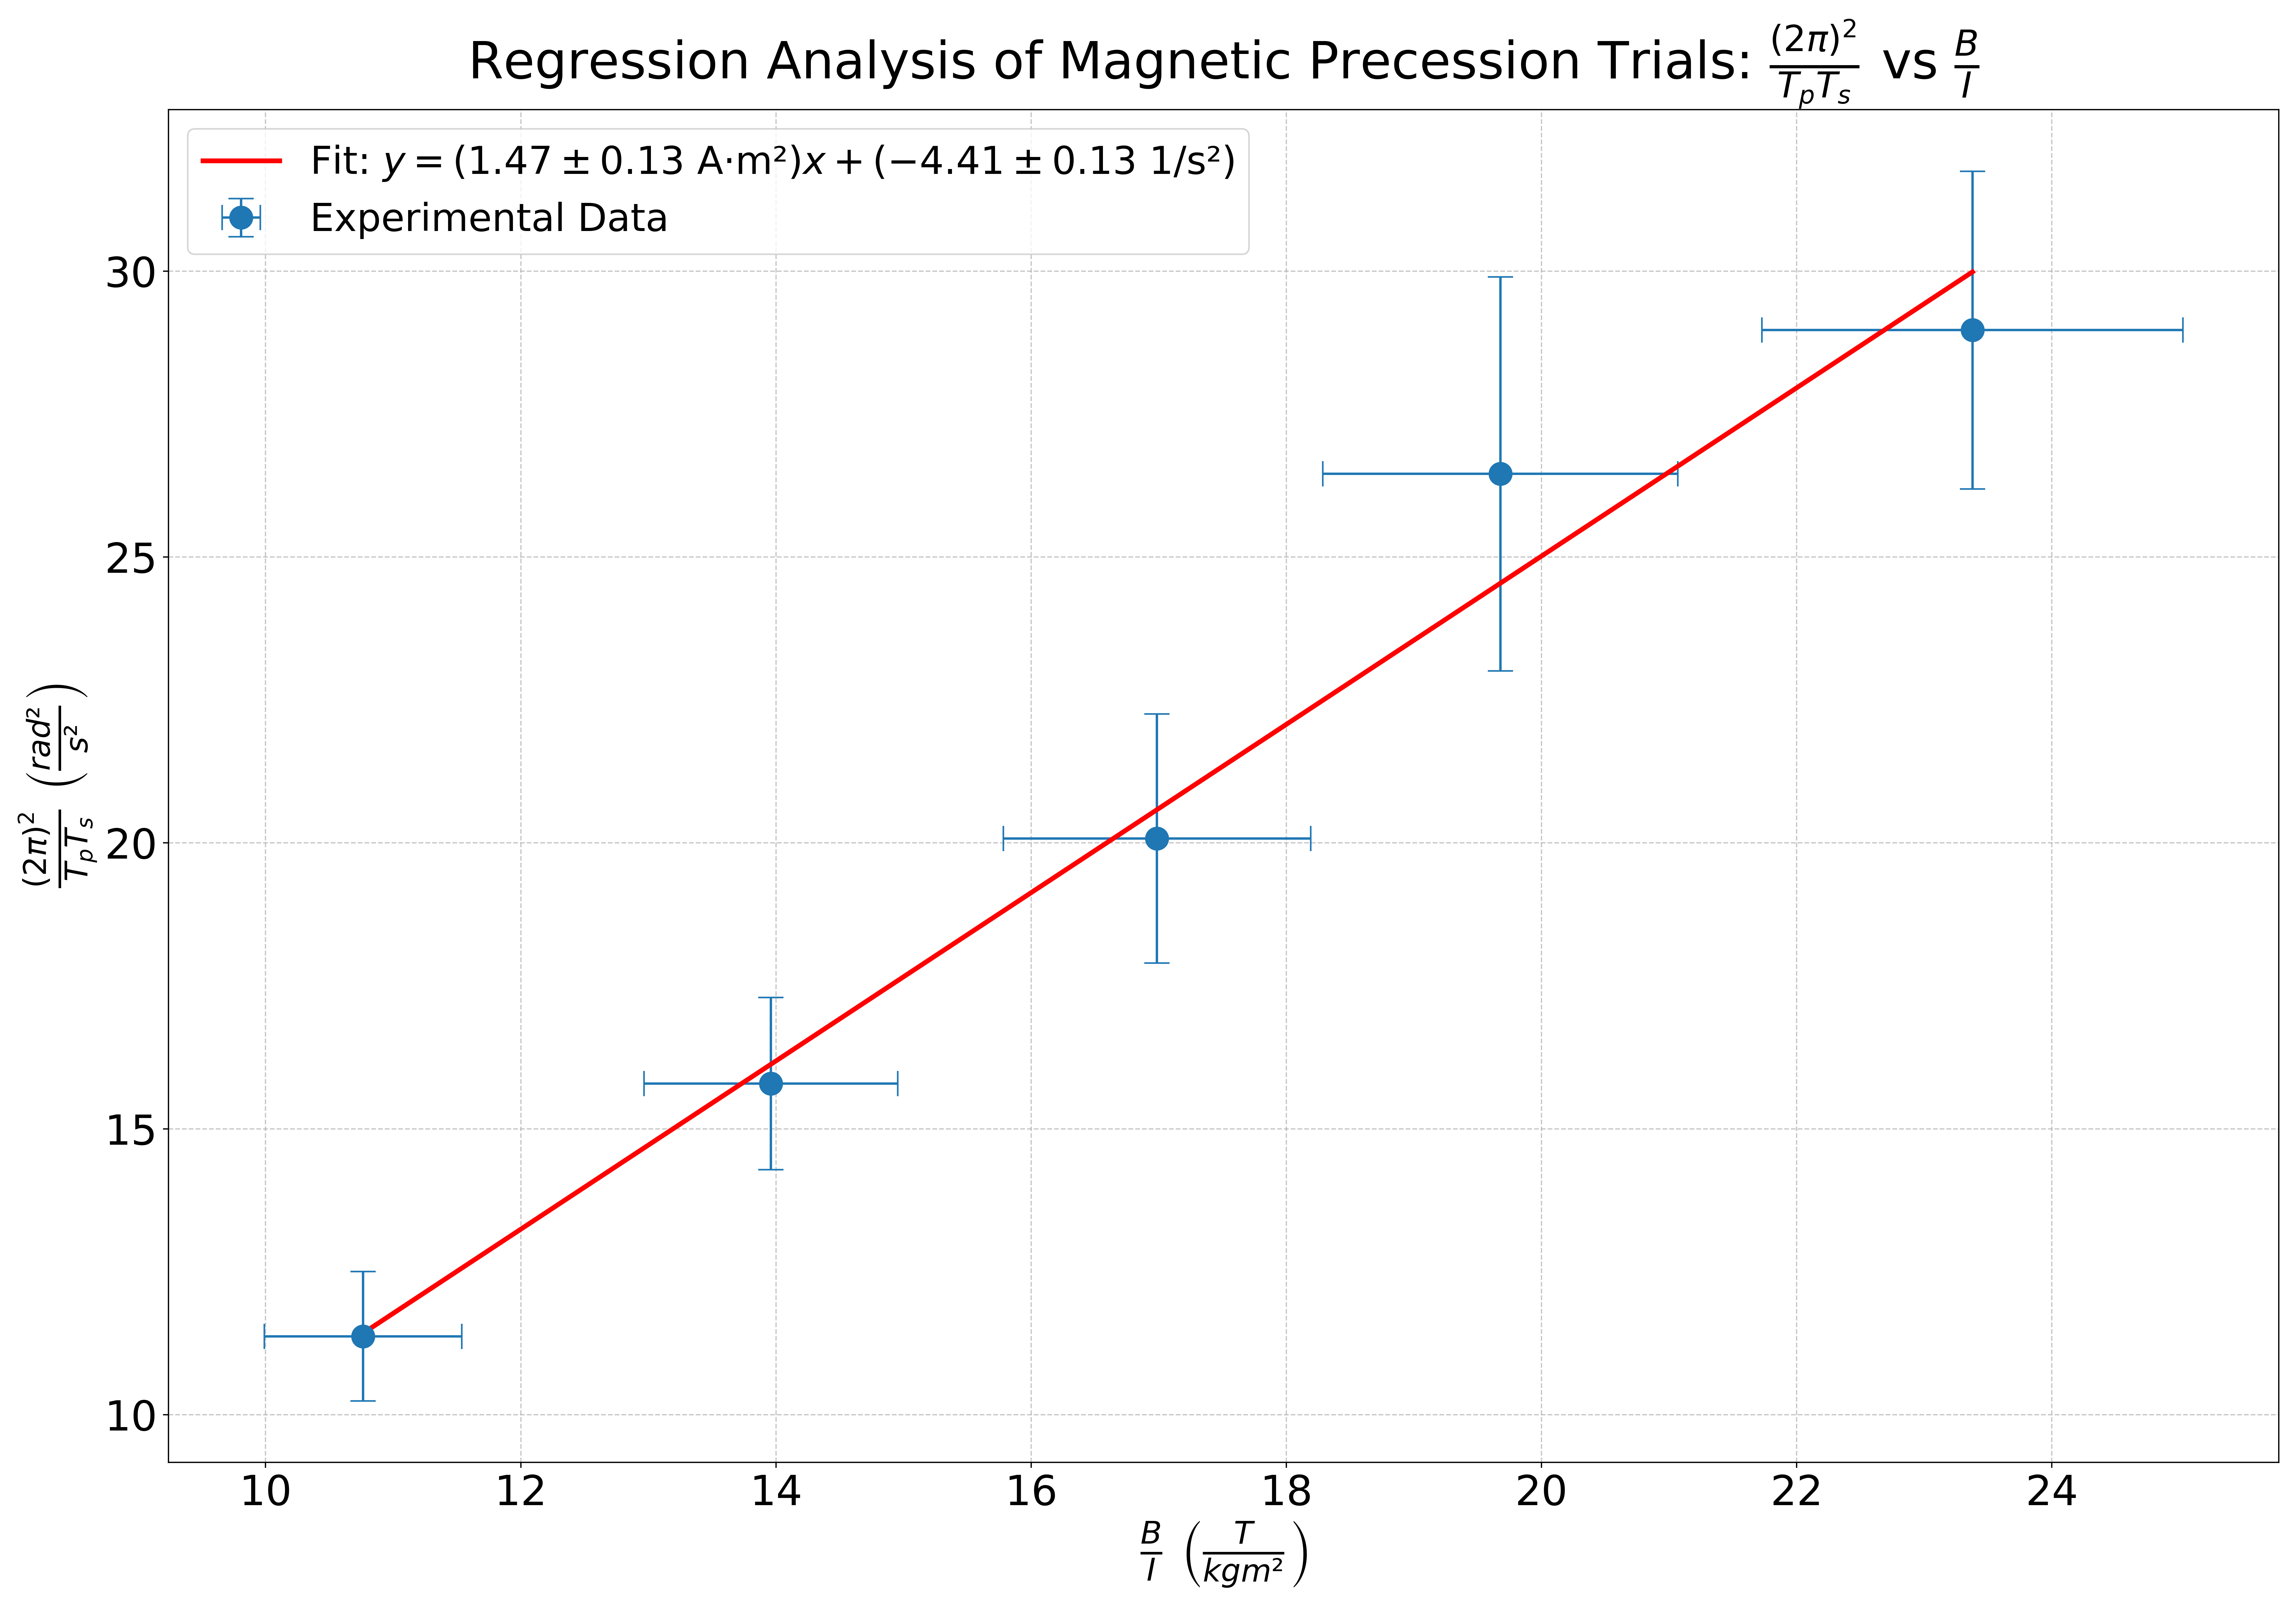
\includegraphics[width=1.0\textwidth]{../magnetic_precession_trials.png}
  \caption{A plot of $\frac{(2\pi)^2}{T_p T_s}$ against $\frac{B}{I}$
    for the magnetic precession experiment.
    The linear regression fit is shown in red, with associated data
  points from Table \ref{tab:results} in blue. Origin not shown.}
  \label{fig:prec_lr_plot}
\end{figure}

A pointwise analysis of the data is also performed, yielding one
value of $\mu$ per trial per experiment (harmonic motion and
precession). These values are organized in Table \ref{tab:pointwise_results}.
A mean and standard-deviation-of-mean analysis is performed, yielding
$\mu$-values of $(1.577 \pm 0.021)$ A $\cdot$ m$^2$ and $(1.19 \pm
0.05)$ A $\cdot$
m$^2$ from the harmonic motion and precession
experiments, respectively. These are not consistent with each other.
However, the value of $\mu$ from
the pointwise analysis for the harmonic motion experiment is
consistent with the values of $\mu$ from the linear regression
analysis--suggesting that the precession experiment deserves futher
attention. Pointwise values of $\mu$ in comparison with
the mean values are organized in Figures \ref{fig:pointwise_comparison_sho} and
\ref{fig:pointwise_comparison_prec}.

\begin{table}[H]
  \centering
  \begin{tabular}{c c c}
    \hline
    Current (A) ($\pm$ 0.01 A) & $\mu$, SHO (A $\cdot$
    m$^2$) & $\mu$,
    Precession (A $\cdot$ m$^2$) \\
    \hline
    2.00 & $1.62 \pm 0.12$ & $1.24 \pm 0.15$ \\
    1.75 & $1.56 \pm 0.12$ & $1.34 \pm 0.20$ \\
    1.50 & $1.56 \pm 0.12$ & $1.18 \pm 0.15$ \\
    1.25 & $1.52 \pm 0.12$ & $1.13 \pm 0.13$ \\
    1.00 & $1.63 \pm 0.12$ & $1.06 \pm 0.13$ \\
    \hline
  \end{tabular}
  \caption{Values of the dipole strength $\mu$ computed per current
  value per experiment.}
  \label{tab:pointwise_results}
\end{table}

\begin{figure}[H]
  \centering
  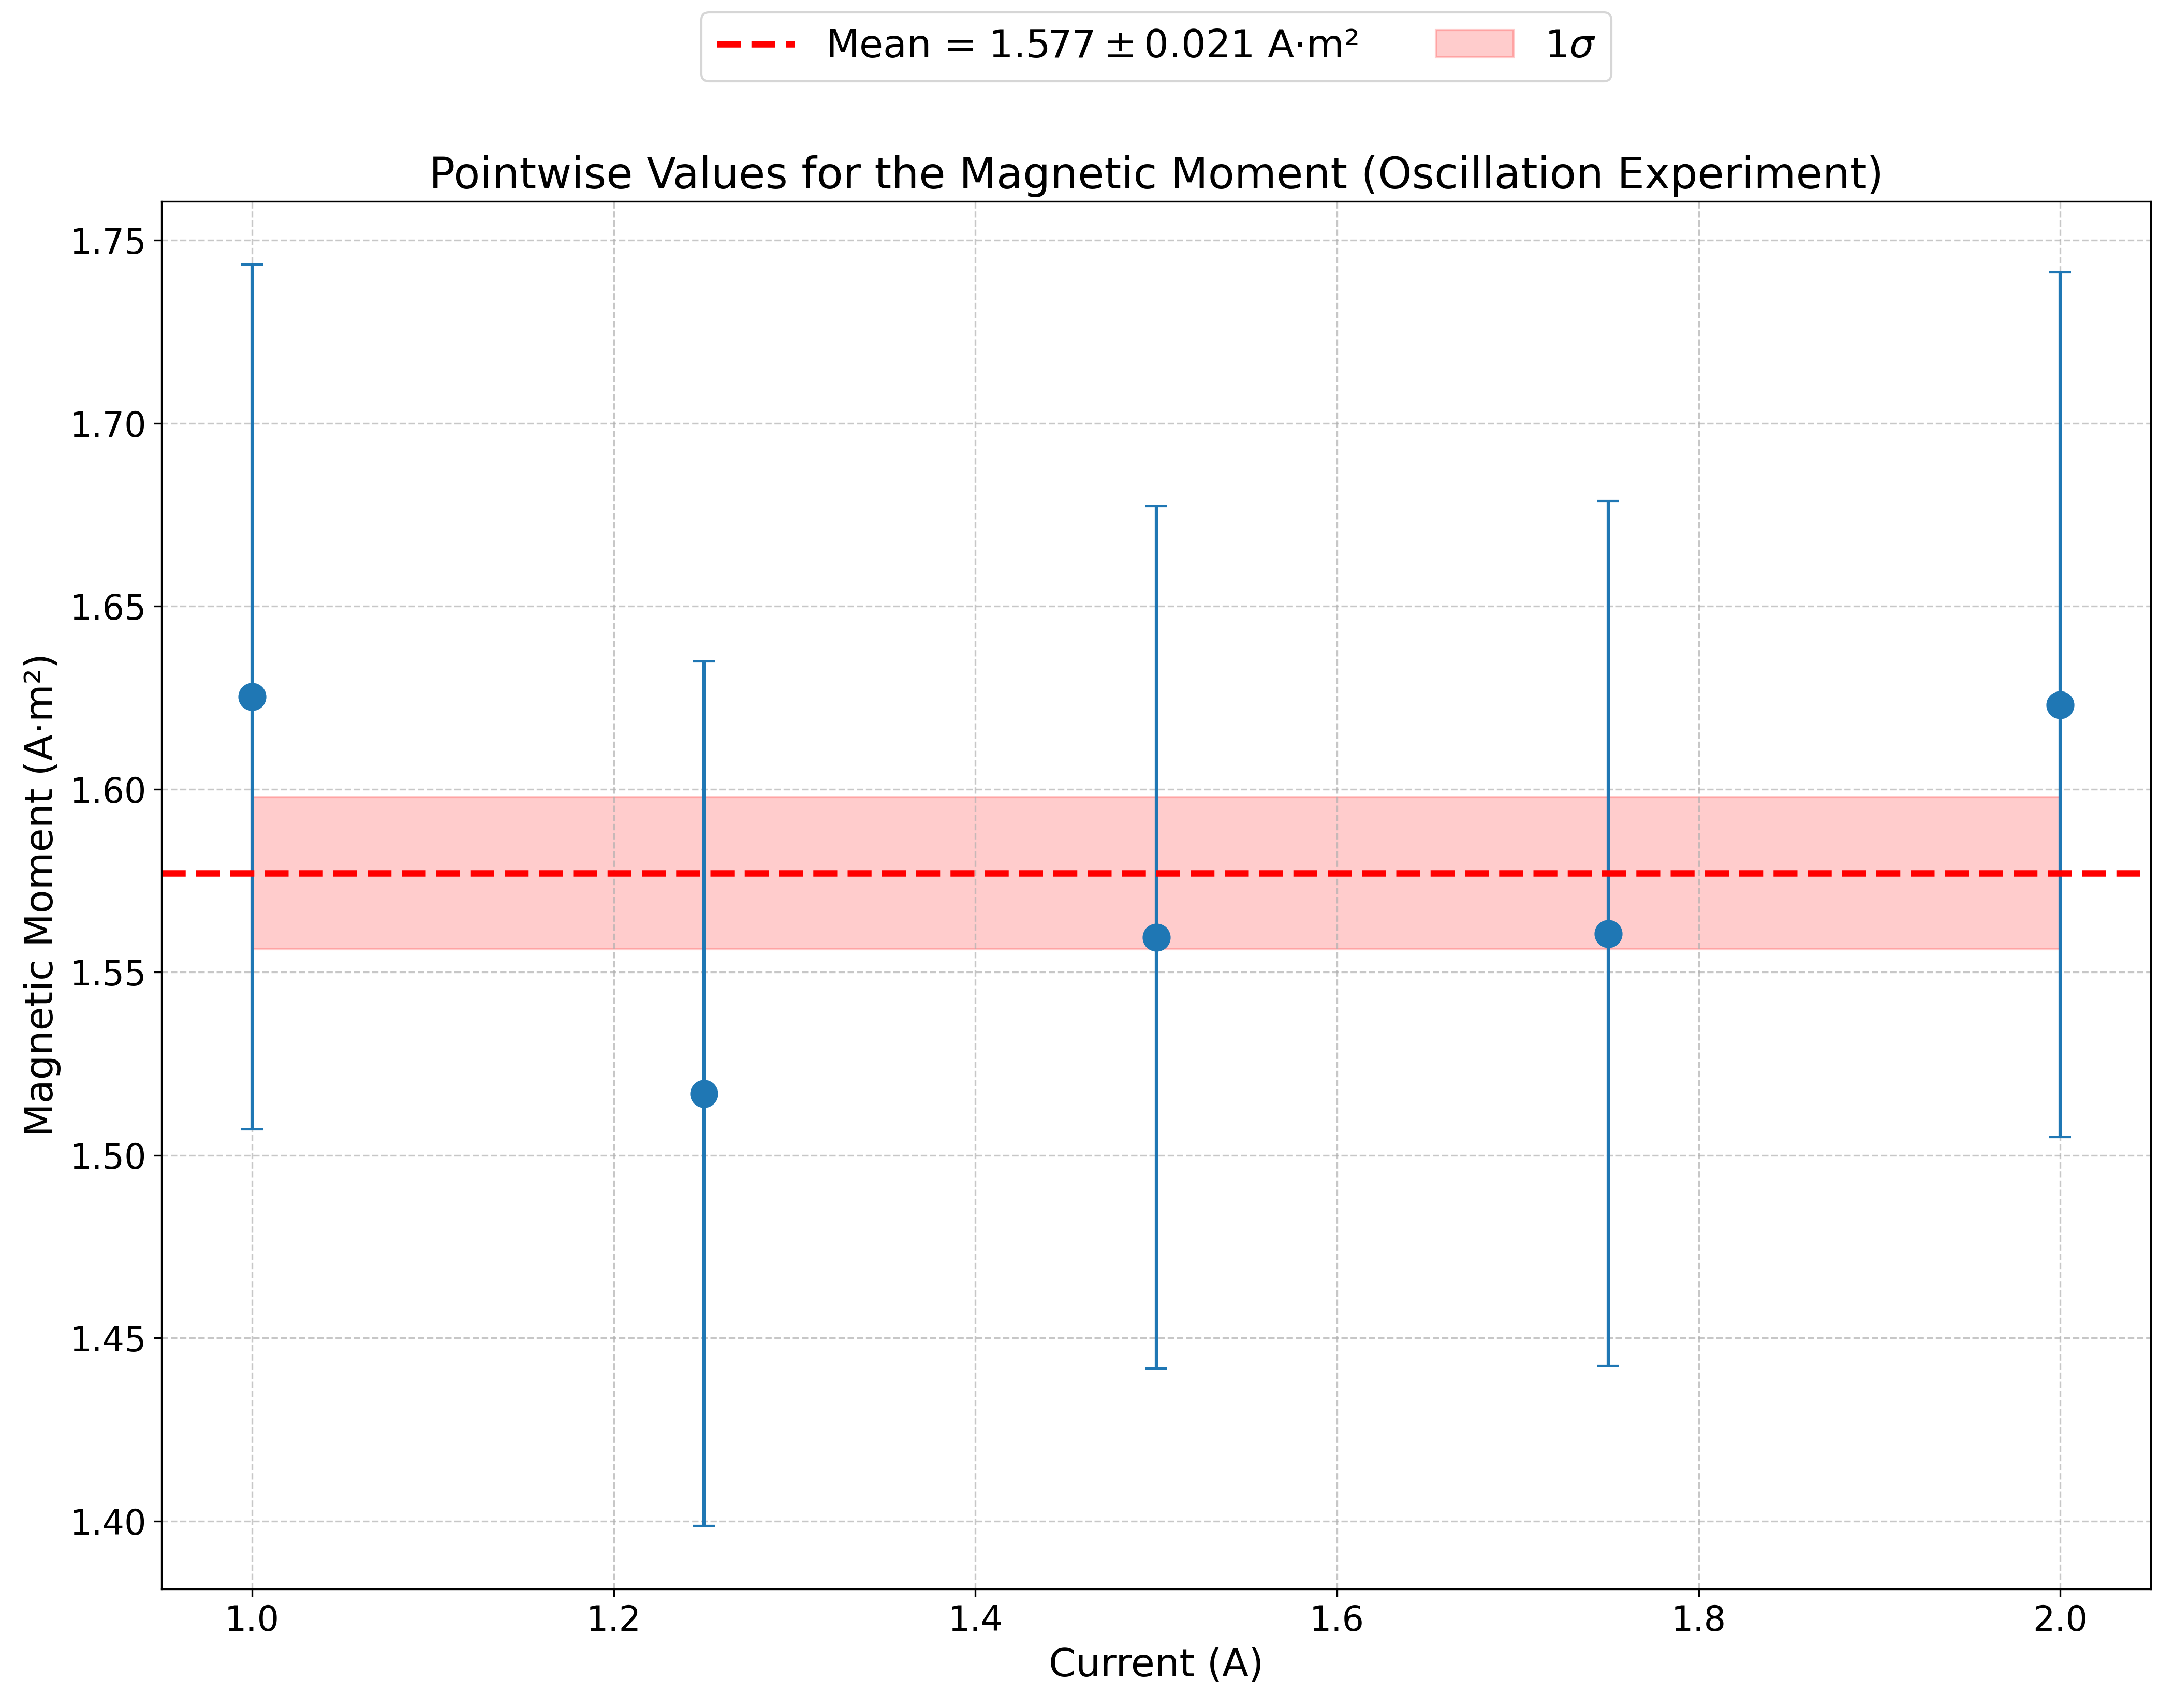
\includegraphics[width=1.0\textwidth]{../mu_sho_plots.png}
  \caption{A plot resulting from the pointwise analysis of the simple
    harmonic motion experiment. The best estimate (mean) is indicated
    with a red dashed line, with the 1$\sigma$ SDOM uncertainty
    interval shaded in red. Points from Table
  \ref{tab:pointwise_results} are shown in blue. Origin not shown.}
  \label{fig:pointwise_comparison_sho}
\end{figure}

\begin{figure}[H]
  \centering
  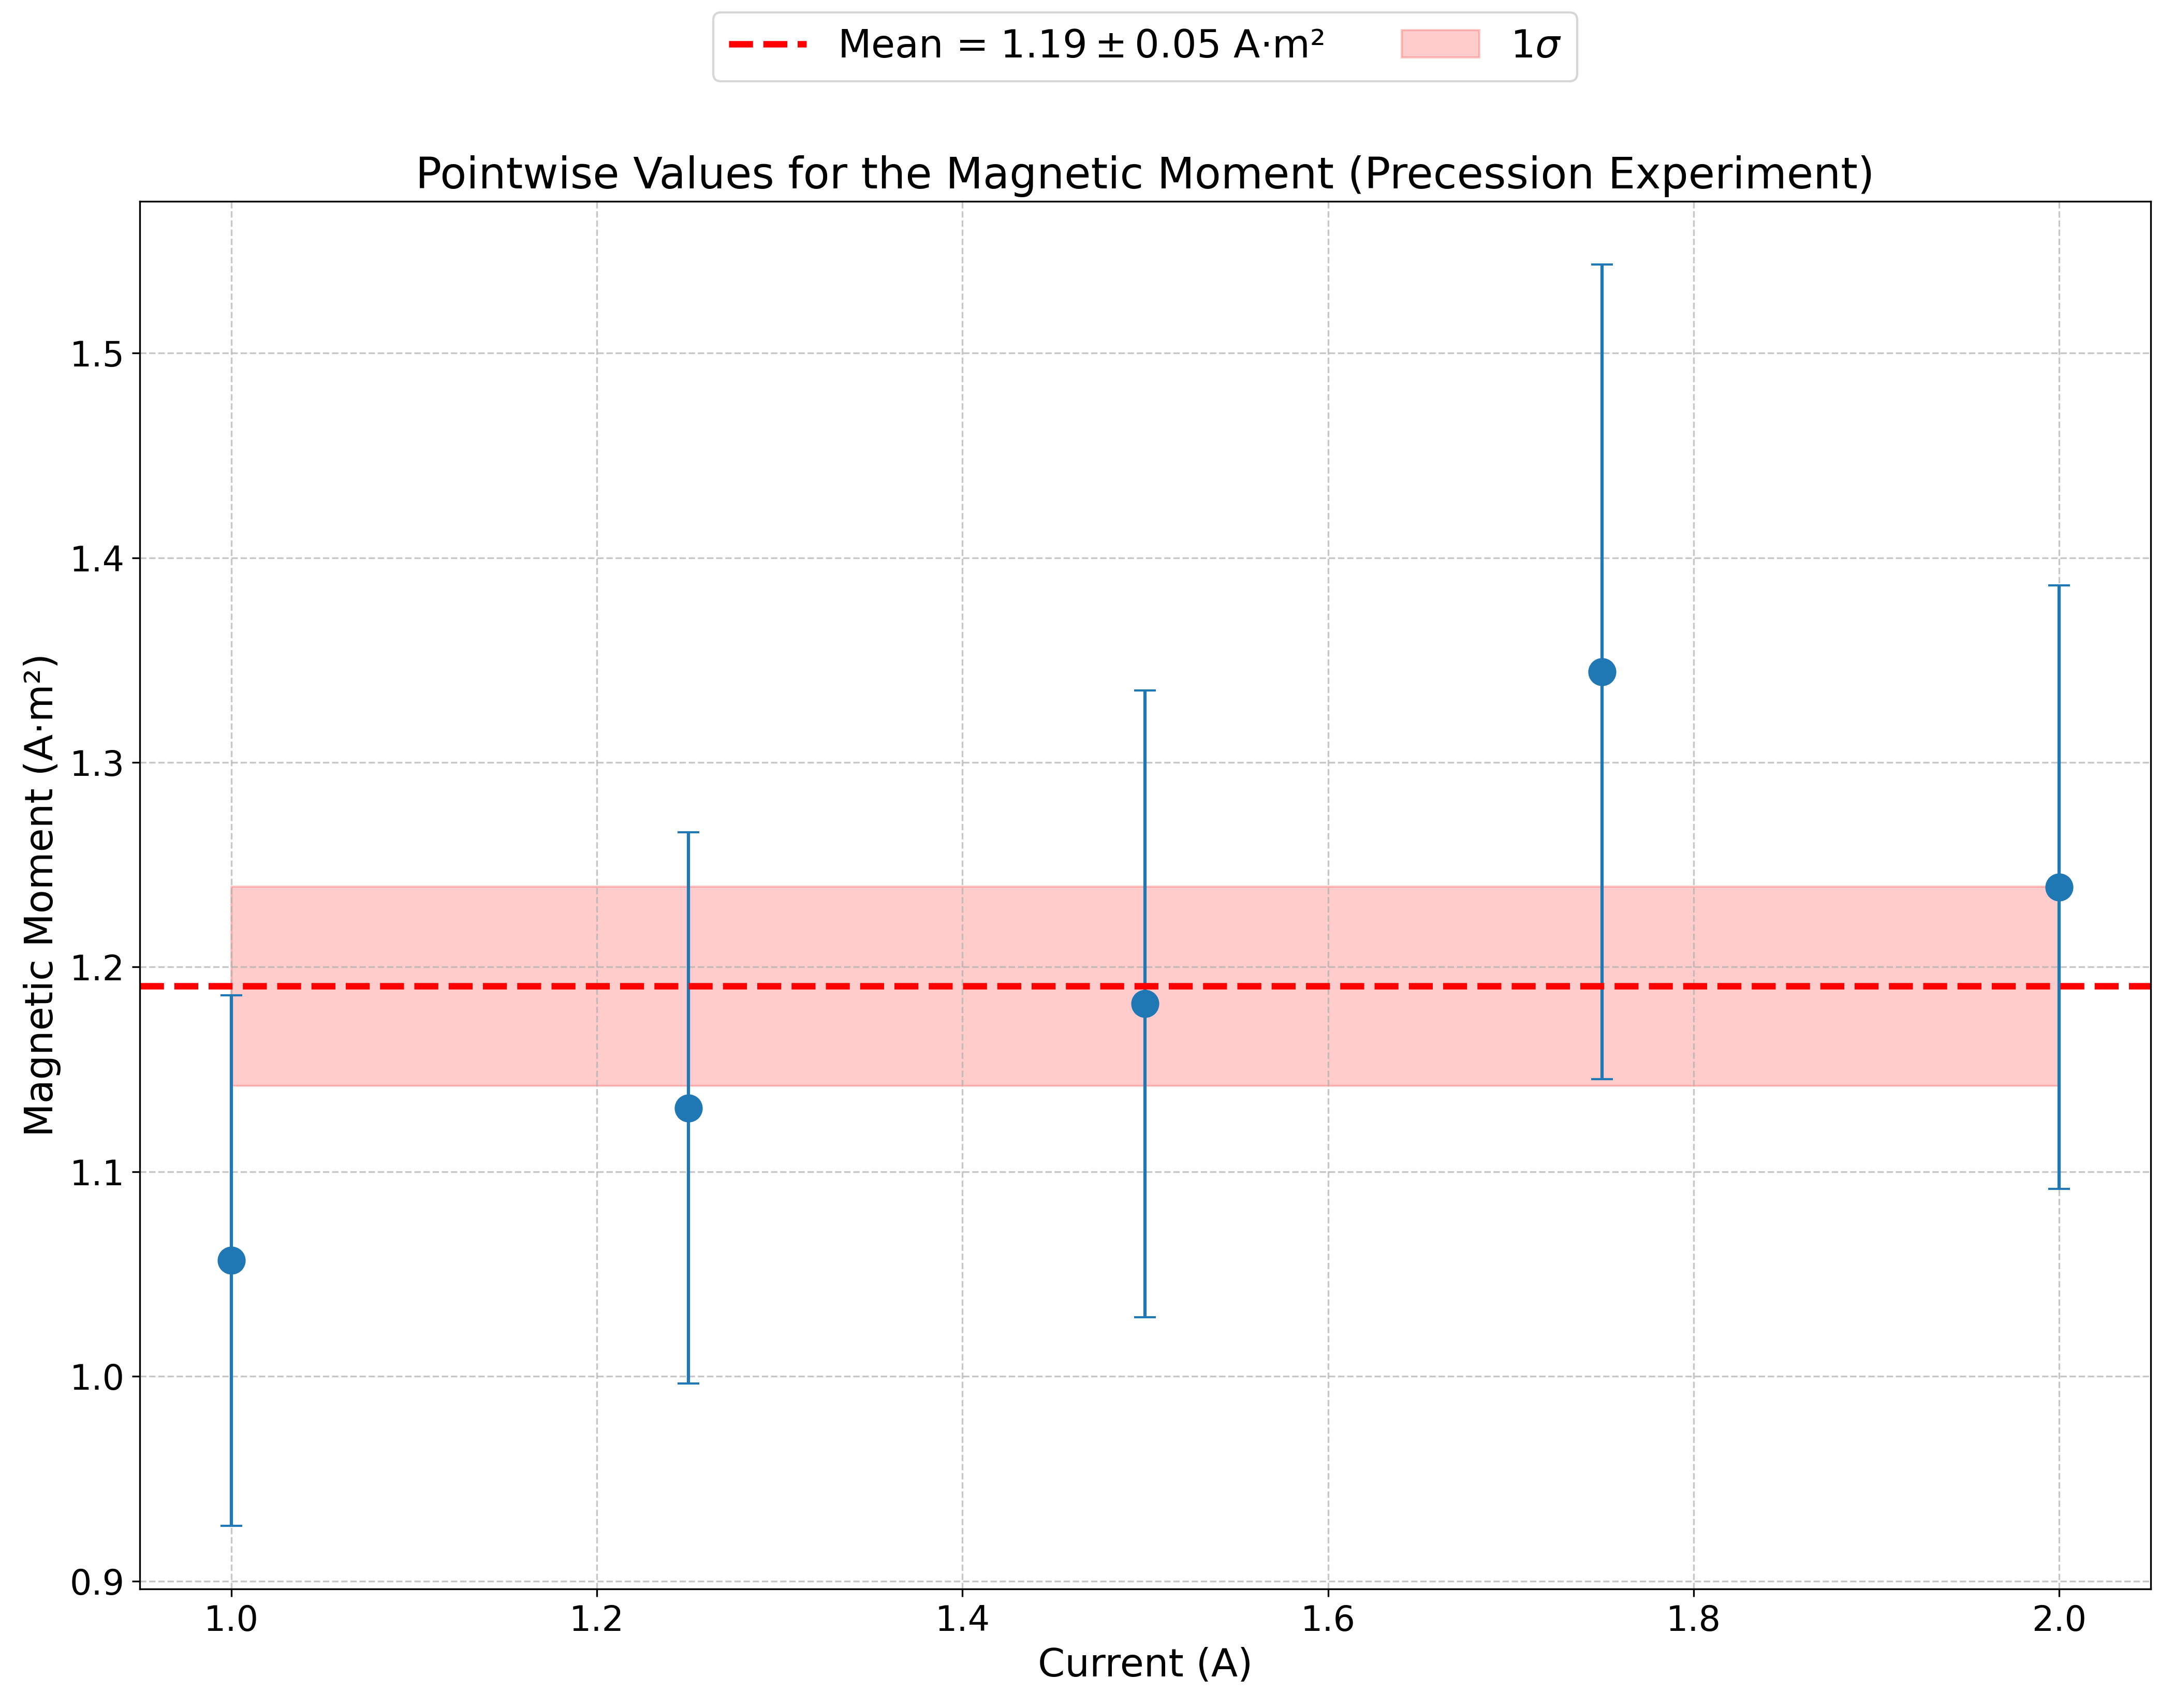
\includegraphics[width=1.0\textwidth]{../mu_prec_plots.png}
  \caption{A plot resulting from the pointwise analysis of the magnetic
    precession experiment. The best estimate (mean) is indicated
    with a red dashed line, with the 1$\sigma$ SDOM uncertainty
    interval shaded in red. Points from Table
  \ref{tab:pointwise_results} are shown in blue. Origin not shown.}
  \label{fig:pointwise_comparison_prec}
\end{figure}

\section{Conclusion and Discussion}

Three experiments are conducted to investigate the behaviors of magnetic dipoles
under the influence of torques produced by external magnetic fields.
The first two
obtain experimental values of the dipole strength $\mu$ from the
simple harmonic motion
and magnetic precession of the dipole in the magnetic field. The
simple harmonic motion experiment
yields $\mu = (1.63 \pm 0.08)$ A $\cdot$ m$^2$ from linear regression
and $\mu = (1.577 \pm
0.021)$ A $\cdot$ m$^2$ from pointwise analysis. The magnetic
precession experiment
yields $\mu = (1.47 \pm 0.13)$ A $\cdot$ m$^2$ from linear regression
and $(1.19 \pm 0.05)$ A $\cdot$ m$^2$
from pointwise analysis.

\vspace{1em}

The inconsistency between the magnetic precession pointwise results
and the three other results
encourages investigation into sources of inaccuracy in the precession
experiments. The method used for obtaining $\omega_s$ readings from
the tachometer is suspect; it is possible that the decay of the
dipole's speed is not strictly linear, causing a deviation of an
ideal estimate of $\omega_s$ from the average value of $\omega_s$ on
the time interval of measurement. The dipole
itself also disturbs the magnetic field produced by the coils once
introduced, potentially invalidating readings of the magnetic field
strength made before placing the dipole in the platform. Measurements
of the precession period also could have been made more robust by
averaging over several trials or by using a more precise method for
timing, such as a video camera instead of a clock.

\vspace{1em}

Across all experiments, the gravitational torque acting on the dipole
contributes to discrepancies between the experimental and true values
of $\mu$. Due to the cavity created by embedding the magnet in the
dipole, the dipole has a non-uniform mass distribution and thus the
gravitational force does not act directly along the dipole's axis of
rotation or oscillation. Earth's magnetic field also contributes
a slight horizontal magnetic field component at the dipole's
position, as do imperfections in the alignment of the coils with the
horizontal plane.

\vspace{1em}

A third experiment investigates the spin flip mechanism of the dipole.
Qualitatively, the torque produced by the transverse magnetic field
is observed to be in line with the theoretical prediction, and the
dipole's orientation is successfully flipped.

\bibliographystyle{plain}
\bibliography{references}

\end{document}
